\documentclass[10pt]{article}
\usepackage{neurips_preprint}
\usepackage[numbers,sort&compress]{natbib}
\usepackage{graphicx}
\usepackage{booktabs}
\usepackage{amsmath}
\usepackage{enumitem}
\usepackage{xcolor}
\usepackage{algorithm}
\usepackage[noend]{algpseudocode}
\algrenewcommand\algorithmiccomment[1]{\hfill{\color{black!55}\(\triangleright\) #1}}
\usepackage[colorlinks=true,linkcolor=blue!50!black,citecolor=blue!50!black,urlcolor=blue!50!black]{hyperref}

\setlist{itemsep=1pt,topsep=2pt}
\preprintnote{Preprint. Work in progress, November 2026.}

\title{Appeasing the Machine Spirit:\\Two Rites of RLHF in In-Context Learning\\for Predicting and Preventing Playtest Notes}

\author{Souradeep Nanda\\
  \normalfont Unemployed Bum}

\begin{document}
\maketitle

\begin{abstract}
A solo developer of an open-world soulslike game plays each new build and writes a list of notes. We ask whether a language-model agent can predict that list from the todo the build was made from, and then change the todo so the list comes back empty. We frame both as learning with no weight updates. The ``weights'' are one plain-text memory file, the data are sixteen git-tagged pairs of todo and playtest list, and every epoch is run by a fresh agent, so the file is the only thing carried forward. The \emph{First Rite} trains the memory on past pairs; the \emph{Second Rite} freezes it and optimises the todo against it, as one would optimise an input against a frozen network. On the training pairs, accuracy rose from 5.5\% to 21.1\% of notes caught over four epochs. But a fixed scorer found that most of the gain was recall: the memory had stored the labels. With recall removed the curve was flat from epoch~2, and a held-out track converged near 3\%. Reading the raw earlier lists predicted held-out notes five times better than any distilled rule set. A memory rewritten as general do/don't pairs, with no past notes in it, caught 5.7\% with zero recall, and its misses point to a line budget, not missing knowledge. Against a baseline with no memory, that is 2.5 times as many held-out notes; against a baseline that only reads the raw history, it is 2.9 times fewer. The Second Rite cut the forecast issues left in the todo from 176 to 32 over five rounds (82\% fewer, and 94\% fewer on its own fixes), though only a real playtest can say whether the real list shrinks too. On the first list no part of the pipeline had seen, the forecast the memory prescribes caught 21 of 112 notes (18.8\%), the best share yet. An ablation on that list found run-to-run noise as large as every component's effect: the recipe scored 21 and then 14 on the same inputs, and only pooling several runs raised recall. We report the protocol, the leaks we found, and what transfers.
\end{abstract}

\section{Introduction}

Playtesting is where a game's problems surface, and for a solo developer it's also the bottleneck: every note costs a play session, and many notes repeat. Over one month of development of \emph{The Good Vet}, a Unity vet game with soulslike fights, the developer wrote sixteen playtest lists against sixteen states of a todo file. Each list was triaged back into the todo, built, and played again. Both files live in git, so the history pairs each todo with the list it produced.

That history is a small supervised dataset of one person's reactions. It invites two questions. Can an agent read a todo and predict the notes the developer will write? And if it can, can it rewrite the todo so those notes never need writing?

We answer both with in-context learning only. Nothing is fine-tuned. The learnt state is a markdown file in the agent's memory directory. We call the procedure \emph{RLHF in ICL}: the human feedback is the developer's own notes, the policy is the forecast, and the update is a rewrite of the memory file. Following the developer, we call the two procedures \emph{rites}. The First Rite trains the memory, and the Second Rite applies it. The machine spirit is appeased when the playtest list comes back empty.

Our contributions are:
\begin{itemize}[leftmargin=*]
  \item A protocol that maps training vocabulary onto agent work: memory file as weights, a fresh agent per epoch as \texttt{zero\_grad()}, git tags as the dataset, and a fixed scorer as the metric (Section~\ref{sec:method}).
  \item Evidence that a naive version overfits by storing labels in the memory, and a recall check that exposes it (Section~\ref{sec:results}).
  \item A held-out comparison showing that raw recent history beats distilled rules by about five times on unseen lists.
  \item A label-free memory written as contrastive do/don't pairs, its frozen test, and an analysis of what it misses and why.
\end{itemize}

\section{Related work}

\paragraph{Learning in the context.} In-context learning goes back to \citet{brown2020language}, and it keeps improving with hundreds of examples in the prompt \citep{agarwal2024manyshot}. RLHF \citep{ouyang2022training} trains weights from human preferences. Here the preferences are free-text notes, and only the context moves.

\paragraph{Memories that learn.} Agents that improve by writing reflections into their context are studied as verbal reinforcement \citep{shinn2023reflexion} and as optimisation through text \citep{yuksekgonul2024textgrad, yang2023opro, khattab2023dspy}. The closest to our First Rite update a persistent memory between tasks:
\begin{itemize}[leftmargin=*]
  \item ExpeL distils insights from successes and failures, edits them only through add, upvote, downvote and edit operations, and also recalls whole past examples \citep{zhao2024expel}.
  \item Dynamic Cheatsheet keeps a self-curated memory at test time, and its stronger variant retrieves the most similar past inputs with their solutions \citep{suzgun2026dynamic}.
  \item GEPA evolves prompts by reflecting on traces, and keeps a Pareto front of candidates in place of a single best \citep{agrawal2026gepa}.
  \item ACE treats the context as a playbook of itemised bullets with helpful and harmful counts, changed only by small deltas \citep{zhang2026ace}. It names the failure our First Rite showed: rewriting the whole context each step collapses it. In their case the context fell from 18,282 tokens to 122, and accuracy fell below the no-memory baseline.
\end{itemize}
Our First Rite differs in its data, one developer's real playtest notes, and in its evidence. Its training curve rose by storing the labels in the memory. A held-out track and a recall count were what exposed it.

\paragraph{Personal prediction from history.} PRELUDE learns a user's latent preferences from their edits. Its CIPHER algorithm retrieves the preferences inferred for the most similar past contexts and combines them \citep{gao2024aligning}. LaMP shows retrieval from a user's own profile helps personalisation \citep{salemi2024lamp}. Both fit our finding that the raw earlier lists predict a held-out list better than any distilled rule set. In software engineering, faults cluster in time and place: a cache of recently fixed or changed files, about a tenth of a project, held 73--95\% of later faults \citep{kim2007predicting}. That is the pattern behind the developer's ``fixed, and back'' notes. Retrieval with ensembled forecasts approaches the human crowd in event forecasting \citep{halawi2024approaching}. Our forecasts were single runs.

\paragraph{Playtesting.} LLM agents already test games for crashes and coverage \citep{zhao2025towards, wang2025leveraging}, and their scores correlate with the difficulty humans report \citep{xiao2024llms}. We found no work that predicts a player's own notes, which is what the rites do.

\paragraph{Refinement and judging.} Refining a model's output with its own feedback gains most in the first one or two rounds \citep{madaan2023selfrefine}. The Second Rite's counts fell fastest in its first rounds too. Its shape is borrowed from input optimisation against a frozen network \citep{szegedy2014intriguing}: the model is held fixed and the input moves to reduce a loss. Using a model to grade a model's output is common practice \citep{zheng2023judging}. But a judge favours text from its own family \citep{panickssery2024llm}, and our forecaster and scorer are the same family. We used one fixed grader across all runs, so scores compare even though the grader may be biased.

\section{Setting}
\label{sec:setting}

\paragraph{Data.} Sixteen playtest lists, written between 2026-10-01 and 2026-11-02, each paired with the todo the build was played against. A pair is two git tags: \texttt{todo/NN} at the commit the list was played against, and \texttt{playtest/NN} where the list is complete. Lists often took several commits, and early ones were committed together with their triage, so tags were needed to make the pairs exact. Each list was also rewritten with clean grammar and one issue per line, tagged \texttt{playtest-rewritten/NN}. Nothing was added or dropped: 551 original lines became 575. Pairs 02--16 are scored, which gives 564 notes. Pair 01 has no earlier history.

\paragraph{The notes.} The developer's notes are concrete. They name the thing, what's wrong with it, and usually what they want (``Bloat looks like GI upset; make it puff up and explode''). Lists run from 6 notes after a small fix build to 85 after a large content pass. Many notes repeat earlier ones, and many are wishes borrowed from games the developer plays.

\paragraph{Metric.} For each real note, a forecast scores 1 if one of its lines names this thing and this problem, closely enough that a ``watch for this'' line on the todo would have caught it. Otherwise it scores 0. One line may match several notes. The headline number is notes caught out of notes written. False alarms don't count against a forecast, as a predicted problem the developer didn't write may be one they missed.

An early lenient rubric also gave half credit for ``the right kind of problem in the right area''. It made vague lines look strong, and flipped the ranking of two forecast sets: 224 against 207.5 under it, 54 against 62 under the strict rubric. The developer's objection settled it: ``I never write crude and vague lines like `case fights need tuning'. What tuning?'' All numbers below are strict. The lenient rubric's failure is a cousin of the brevity bias ACE reports in prompt optimisation, where prompts drift toward short, generic instructions \citep{zhang2026ace}: credit for a category rewards a line that commits to nothing.

\paragraph{The scorer.} A model grades the forecasts, as is common practice \citep{zheng2023judging}. Model judges carry known biases, and one matters here: a judge favours text from its own family \citep{panickssery2024llm}, and our forecaster and scorer are both Claude. We hold the scorer fixed across every run, so comparisons between runs share whatever bias it has. The strict rubric also narrows the room for judgement: a match needs the same thing and the same problem.

\section{Method}
\label{sec:method}

\begin{table}[t]
  \caption{The vocabulary of the two rites.}
  \label{tab:analogy}
  \centering
  \small
  \begin{tabular}{@{}p{0.27\linewidth}p{0.66\linewidth}@{}}
    \toprule
    Deep learning & The rites \\
    \midrule
    Weights & One markdown memory file, versioned in its own git repository \\
    Dataset & Tag pairs: \texttt{todo/NN} as input, \texttt{playtest-rewritten/NN} as label \\
    Forward pass & An agent forecasts a list from a todo, writing before it opens the label \\
    Loss & Forecast against label, as a count and a written account of misses, wrong directions and false alarms \\
    Backward pass & Aggregating the per-pair losses into patterns \\
    \texttt{optimizer.step()} & Rewriting the memory file \\
    \texttt{zero\_grad()} & A fresh agent each epoch; the file is all that carries over \\
    Checkpoint & A commit and tag in the memory repository \\
    Data leakage & Reading a label before its forecast, or reusing an agent across epochs \\
    Overfitting & Past notes written into the memory \\
    \bottomrule
  \end{tabular}
\end{table}

\begin{algorithm}[t]
  \caption{The First Rite: train the memory on past pairs}
  \label{alg:first}
  \small
  \begin{algorithmic}[1]
    \Require pairs $(t_k, y_k)$ for $k = 2, \dots, K$ (todo, playtest list); commit subjects $s_k$; memory $M_0$; fixed scorer $S$
    \For{$e = 1, 2, \dots$}
      \State $A \gets$ a fresh agent \Comment{\texttt{zero\_grad()}: no context carries over}
      \For{$k = 2, \dots, K$}
        \State $\hat{y}_k \gets A.\textsc{Forecast}(M_{e-1}, t_k, s_k, y_{<k})$ \Comment{written before $y_k$ is opened}
        \State $\ell_k \gets A.\textsc{Loss}(\hat{y}_k, y_k)$ \Comment{a count, and what went wrong in words}
      \EndFor
      \State $g \gets A.\textsc{Aggregate}(\ell_2, \dots, \ell_K)$ \Comment{patterns across pairs}
      \State $M_e \gets A.\textsc{Rewrite}(M_{e-1}, g)$ \Comment{general do/don't pairs; no past notes}
      \State commit $M_e$ \Comment{checkpoint}
      \State $(\mathit{hits}_e, \mathit{recall}_e) \gets S(\hat{y}, y)$ \Comment{same scorer every epoch}
      \If{$\mathit{hits}_e - \mathit{recall}_e$ stops rising, or held-out hits stop rising, or $M_e = M_{e-1}$}
        \State \Return $M_e$
      \EndIf
    \EndFor
  \end{algorithmic}
\end{algorithm}

\begin{algorithm}[t]
  \caption{The Second Rite: freeze the memory, converge the todo}
  \label{alg:second}
  \small
  \begin{algorithmic}[1]
    \Require frozen memory $M$; current todo $T_0$; subjects $s$; every past list $y_1, \dots, y_K$; threshold $\tau$; cap $R$
    \For{$r = 0, 1, \dots, R - 1$}
      \State $A \gets$ a fresh agent \Comment{reads $T_r$ as it now stands}
      \State $\hat{y} \gets A.\textsc{Forecast}(M, T_r, s, y_{1..K})$ \Comment{as if every open box were built as written}
      \State $N \gets \{\, n \in \hat{y} : T_r \text{ doesn't already cover } n \,\}$ \Comment{the loss}
      \State $T_{r+1} \gets \textsc{Fold}(T_r, N)$ \Comment{a box, a watch line, a tightened box, or a decision}
      \State commit $T_{r+1}$
      \If{$|N| < \tau$}
        \State \Return $T_{r+1}$ \Comment{converged: the forecast finds nothing new}
      \EndIf
    \EndFor
    \State \Return $T_R$
  \end{algorithmic}
\end{algorithm}

\paragraph{The First Rite: train the memory.} Algorithm~\ref{alg:first} gives the loop. Each epoch, a fresh agent (Claude Opus 5.5 at high effort) reads the memory file and walks pairs 02--16 in order. For each pair it reads only the todo and the commit subjects since the last list. It writes at most twelve forecast lines to a file, then opens the label and writes a loss: the self-score, and what it predicted against what came. After the last pair it aggregates its losses and rewrites the memory file, then commits it. Inputs are prepared as files, so no agent reads the game's codebase. One persistent agent scores every epoch, so the numbers compare. It also estimates \emph{recall}: hits that restate a note from the scored list itself, with a detail no input gives.

Three choices follow earlier work. The loss is written in words as well as counted, because language feedback carries more than a scalar reward: GEPA's reflection beat reinforcement learning with far fewer rollouts \citep{agrawal2026gepa}, and TextGrad treats such feedback as a gradient \citep{yuksekgonul2024textgrad}. The memory is a store of verbal lessons, as in Reflexion \citep{shinn2023reflexion}. And it keeps its own score history, much as OPRO's meta-prompt keeps past solutions with their scores \citep{yang2023opro}. An epoch over a fixed training split followed by evaluation matches ACE's offline adaptation \citep{zhang2026ace}.

\paragraph{Validation.} Beside the main loop, a second track starts from an empty memory, trains on pairs 02--13, and never opens lists 14--16. Each epoch it forecasts 14--16 from the memory as loaded, before training, and the same scorer grades those forecasts. That curve is the honest one. Forecasting benchmarks keep test questions past a model's knowledge cutoff for the same reason \citep{halawi2024approaching}. Here the cutoff that matters is the memory's: a held-out list must be unseen by every part of the pipeline, the memory included.

\paragraph{The Second Rite: converge the todo.} Algorithm~\ref{alg:second} gives the loop. The memory is frozen. A fresh agent reads the memory, the current todo, and every past list raw. It forecasts the developer's notes on the build the todo describes, as if every open box were built as written. Each new forecast line is folded into the todo, as a fix box, a ``watch'' line on an existing box, a tightened box, or a decision with a default. Lines that need no building are dropped. The next round is a fresh agent on the new todo. The rite stops when a round adds almost nothing. The loss here is the count of new issues, and the input, not the model, is what moves. The loop resembles Self-Refine, where a model critiques and revises its own output \citep{madaan2023selfrefine}, with two differences. The critic is a frozen memory forecasting another person's reaction, and the thing revised is a plan of work, not a finished output.

\section{Results}
\label{sec:results}

\begin{figure}[t]
  \centering
  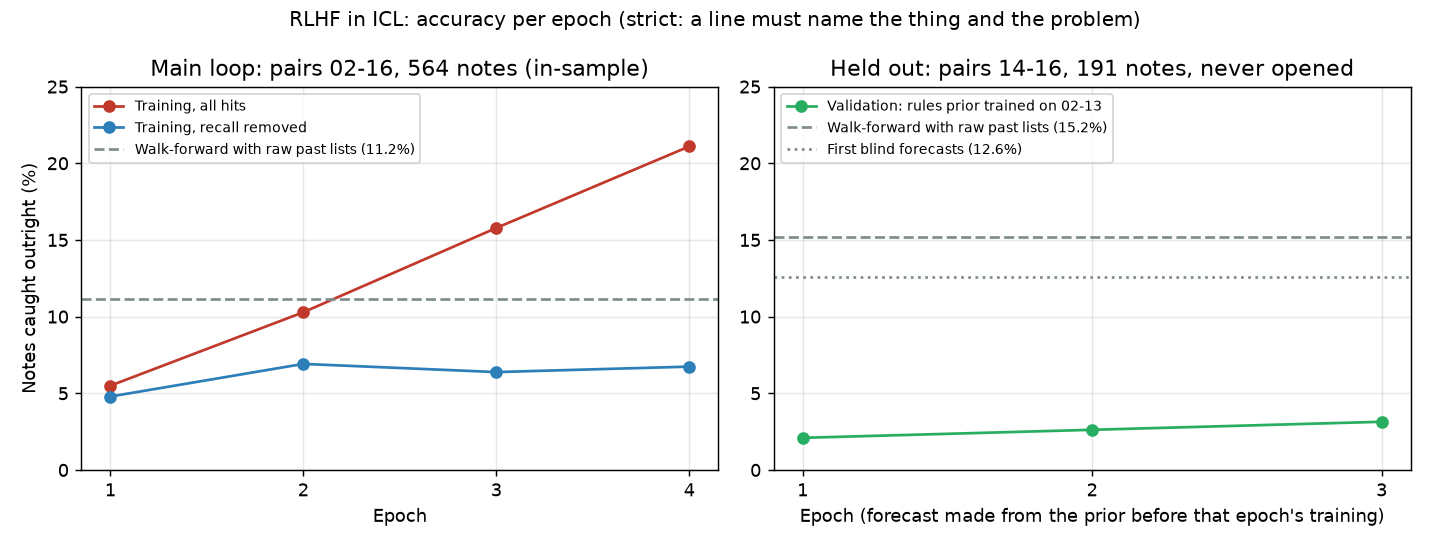
\includegraphics[width=\linewidth]{figures/accuracy.png}
  \caption{Left: the First Rite on pairs 02--16 (in-sample). All hits rise; hits with recall removed are flat from epoch 2. Right: the validation track on held-out pairs 14--16. Dashed lines are agents with the raw earlier lists in context and no rules memory.}
  \label{fig:accuracy}
\end{figure}

\begin{table}[t]
  \caption{Notes caught, strict rubric, one fixed scorer. Training is pairs 02--16 (564 notes). Held out is pairs 14--16 (191 notes), never opened by the validation track. The held-out multiples are against the no-memory baseline (4 notes, 2.1\%). Baselines don't use the First Rite.}
  \label{tab:main}
  \centering
  \small
  \begin{tabular}{@{}lrrr@{}}
    \toprule
    Run & All hits (564) & Recall removed & Held out (191) \\
    \midrule
    Baseline: no memory, no past lists & -- & -- & 4 (2.1\%) \\
    \midrule
    First Rite, epoch 1 & 31 (5.5\%) & $\sim$27 & -- \\
    First Rite, epoch 2 & 58 (10.3\%) & $\sim$39 & -- \\
    First Rite, epoch 3 & 89 (15.8\%) & $\sim$36 & -- \\
    First Rite, epoch 4 & 119 (21.1\%) & $\sim$38 & -- \\
    \midrule
    First Rite, validation epochs 1--3 & -- & -- & 4, 5, 6 (1.0--1.5$\times$) \\
    \midrule
    Baseline: raw earlier lists, no memory & 63 (11.2\%) & 63 & 29 (7.2$\times$) \\
    Baseline: first blind forecasts & 55 (9.8\%) & 55 & 24 (6.0$\times$) \\
    First Rite: frozen do/don't memory, last 3 lists & 32 (5.7\%) & 32 & 10 (2.5$\times$) \\
    \bottomrule
  \end{tabular}
\end{table}

\paragraph{Training accuracy rose, but the gain was memory.} Over four epochs the First Rite climbed from 31 to 119 notes (Table~\ref{tab:main}, Figure~\ref{fig:accuracy}). The fixed scorer flagged that many hits repeated the scored list almost word for word. By epoch~4, about 81 of 119 hits were recall. With recall removed the curve was flat from epoch~2, at about 38. Each epoch's agent had written past notes into the memory: lists of chronic offenders tagged with the lists they came from, per-tool lists of asks, and a ladder of wishes. Those are the labels. A forecaster that reads them is looking things up. The update rule invited it. Each epoch rewrote the whole memory, the monolithic rewrite that ACE shows can collapse a context \citep{zhang2026ace}. Here it drifted the other way, toward stored answers. Methods that change a memory only through small, scored edits, such as ExpeL's add, upvote, downvote and edit operations \citep{zhao2024expel} or ACE's counted bullets, give such drift less room.

\paragraph{Validation converged low.} The validation track, which never saw lists 14--16, caught 4, 5 and 6 of their 191 notes over three epochs. That's within noise of each other, and flat.

\begin{figure}[t]
  \centering
  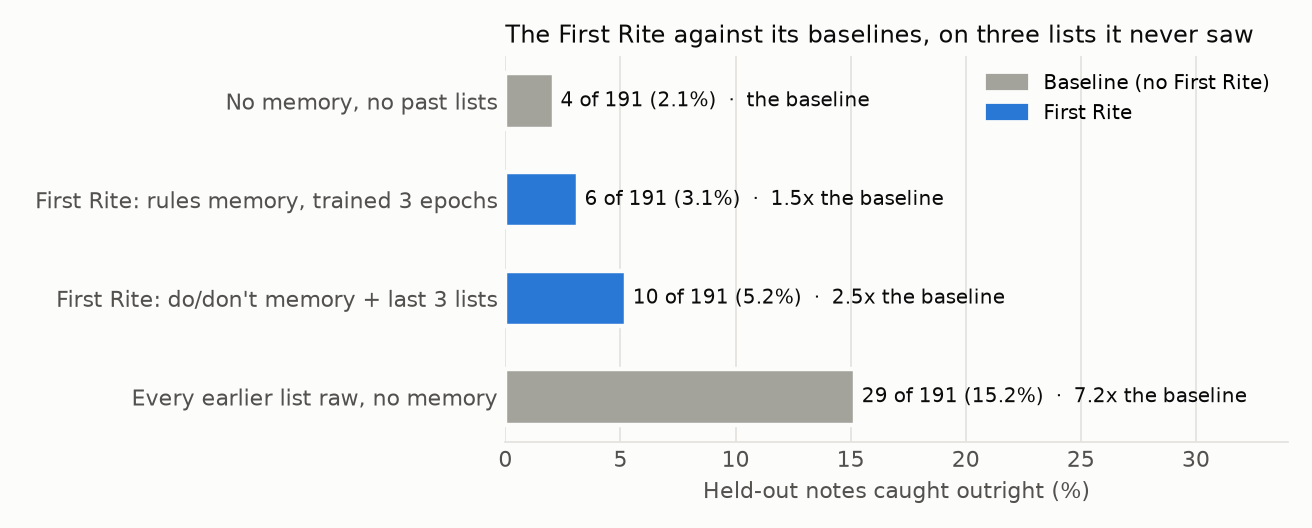
\includegraphics[width=\linewidth]{figures/rite1-baselines.png}
  \caption{The First Rite against two baselines that don't use it, on the 191 notes of held-out pairs 14--16. Grey: no memory and no past lists; every earlier list raw with no memory. Blue: the rules memory trained by the First Rite; the do/don't memory with the last three lists.}
  \label{fig:rite1}
\end{figure}

\paragraph{Against the baselines.} Figure~\ref{fig:rite1} sets the First Rite against two baselines that don't use it. With no memory and no past lists, a forecaster caught 4 of the 191 held-out notes (2.1\%). The First Rite's trained rules caught 6 (3.1\%), 1.5 times that baseline, a 50\% gain. The label-free do/don't memory with the last three lists caught 10 (5.2\%), 2.5 times the baseline, a 150\% gain. The second baseline, every earlier list raw with no memory at all, caught 29 (15.2\%), 7.2 times the first baseline and 2.9 times the do/don't memory. So the First Rite beats having nothing, but not reading the history. The combination the memory now prescribes, its do/don't rules plus every earlier list and no line cap, was scored only by the next playtest (below).

\paragraph{Raw history beats distilled rules.} An agent with no rules memory but with every earlier list in context caught 29 of the same 191 held-out notes: five times the validation track. The notes that come are mostly repeats of named things, half-finished asks, and the next step of a wish. Those live in the raw lists. A rule about them (``fixes checked only by a test come back'') doesn't say which thing will come back. This matches three lines of earlier work:
\begin{itemize}[leftmargin=*]
  \item In-context learning keeps gaining as examples grow into the hundreds \citep{agarwal2024manyshot}, and the whole history here, about 560 notes, fits in one context.
  \item Personalisation works best when it retrieves from the user's own history \citep{salemi2024lamp, gao2024aligning}, and Dynamic Cheatsheet's strongest variant pairs its memory with retrieval of similar past inputs \citep{suzgun2026dynamic}.
  \item In software, faults cluster in time and place, so a small cache of recently fixed files predicts most later faults \citep{kim2007predicting}. The developer's ``fixed, and back'' notes are that locality.
\end{itemize}

\paragraph{A label-free memory.} The memory was rewritten in general terms as contrastive do/don't pairs, each rule stated with its opposite, and with no past notes in it. Like PRELUDE's preference descriptions \citep{gao2024aligning}, it can be read and corrected by the person it models. The developer did both, and their corrections (``this is cheating'', ``dos and donts'') shaped it more than any epoch did. Frozen and tested by a fresh agent with the last three lists in context, it caught 32 of 564 notes with zero recall, and 10 of 191 on pairs 14--16, twice the validation track's best. Its 520 misses split three ways:
\begin{itemize}[leftmargin=*]
  \item 298 were covered by rules the memory already had, with no line left under the twelve-line cap.
  \item 137 could not have been predicted from any input: new ideas, one-off bugs, taste. Writing them in would be overfitting.
  \item 85 pointed to missing rules. Four held across five or more lists and were added: things built from one template get called samey; text gets judged on whether it can be read and found; a fix checked only by a test can be back by the next list; anything needing precision gets asked to be more generous. The rest came from one or two lists and stayed out.
\end{itemize}
The cap was the largest loss, and the developer's view settles how to lift it: a predicted problem that doesn't come up costs nothing, and ``it could be an oversight on my part''. Of the 146 forecast lines that matched no note, the scorer judged 92 to be plausible problems the developer may simply not have written down.

\paragraph{The Second Rite.} From the frozen memory, the current todo and all sixteen lists, a fresh agent forecast 176 notes for the next playtest. Folded into the todo:
\begin{itemize}[leftmargin=*]
  \item 22 were already handled in the code;
  \item 4 were play-only, with nothing to build;
  \item 40 became 35 watch lines on existing boxes;
  \item 90 became 64 fix boxes, each with a check that needs no human player;
  \item 20 wishes became 9 decisions with defaults.
\end{itemize}
Round~1, a fresh agent on the new todo, forecast 87 more lines. It found 79 of them new: 38 risks on boxes that round~0 had just added, 14 more boxes, 16 boxes too vague to come out right, and 11 wishes. Most were faults in round~0's own fixes, as in any iteration where each step adds surface for the next. Round~2 found 44 new items in 51 lines, mostly risks on round~1's additions, and round~3 found 28. Round~4 found 22, but 10 of those came from the game's chapter documents, whose lists of untested parts no earlier round had read. Round~5 read the rest of them and found 32, of which 22 came from the documents and 10 from round~4's own additions. We stopped at the cap of five rounds.

On its own surface the rite converged: the items each round found in the last round's additions fell 79, 44, 28, 12, 10 (Figure~\ref{fig:rite2}). The shape matches self-refinement, where most of the gain comes in the first one or two rounds \citep{madaan2023selfrefine}. Two or three rounds may be enough.

The baseline here is not running the rite: the todo stays as it was, and all 176 forecast issues remain in the build. Against that baseline, the forecasts after each round found 55\%, 75\%, 84\%, 88\% and 82\% fewer new issues. Counting only what each round found in the last round's own fixes, round~5's 10 is 94\% below the baseline. These are issues a forecaster expects, not issues found by play: the reduction says the frozen memory can think of little more to raise, and only the developer's next playtest says whether that holds.

\begin{figure}[t]
  \centering
  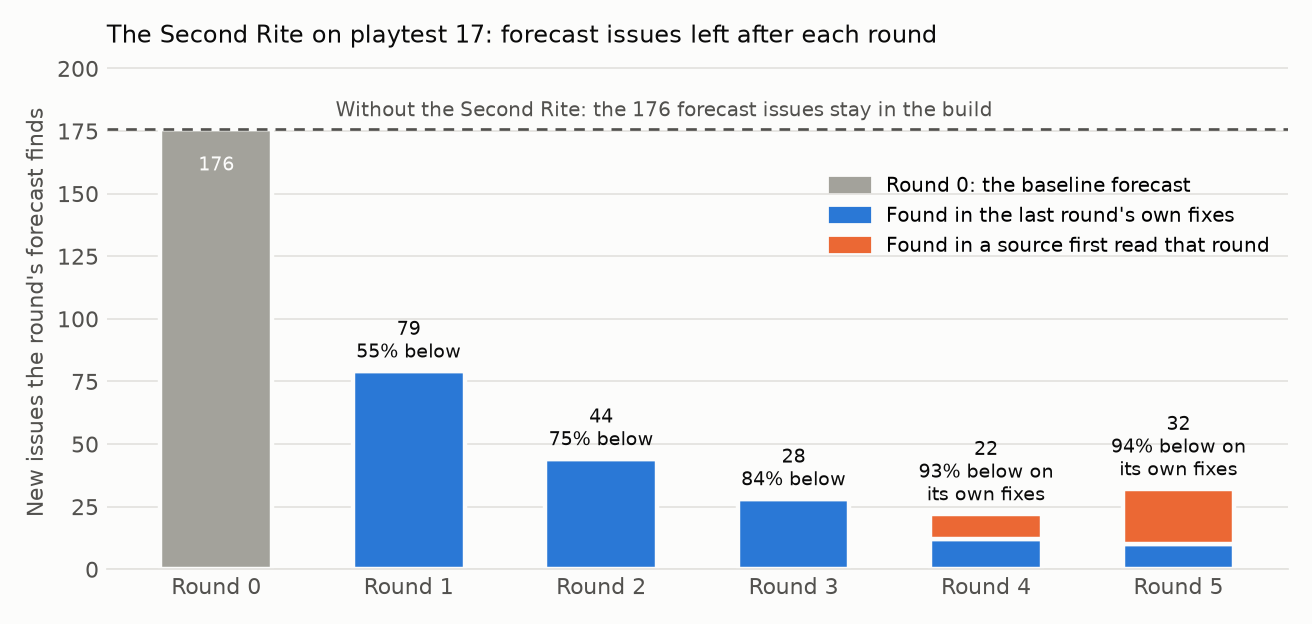
\includegraphics[width=\linewidth]{figures/rite2-rounds.png}
  \caption{The Second Rite on playtest 17: new issues each round's forecast finds, against the baseline of not running it (dashed, 176). Blue: found in the last round's own fixes. Orange: found in a source the round read for the first time (the chapter documents).}
  \label{fig:rite2}
\end{figure} It never reached the stop line of five, because each new source behaved like new data. The lesson is to give round~0 every source at once (the todo, the commit subjects, every past list, and every document that lists untested parts), so later rounds only see their own surface. The last agent's view of what remains is what only play can find: how the new chapters feel, prices, the fixed numbers, run-time placement seen from a player's eye, and a real friend on a real connection. The real test of both rites is the developer's next playtest, which no model has seen.

\paragraph{The first unseen list.} The developer then played the build that round~0 forecast, with section 72 still unbuilt, and wrote list 17: 112 notes. It is the first list no part of the pipeline had seen. Round~0's forecast used what the memory prescribes, the do/don't rules plus every earlier list with no cap on lines. It caught 21 of the 112 notes (18.8\%), with zero recall. That is the best share yet on an unseen list, above the 15.2\% that raw history reached on lists 14--16, though the lists differ. It took 176 lines, of which 20 hit (11\%). Rounds 1--5, which forecast fixes that weren't built, added 2 more notes. Of the list's 8 repeats of old notes, round~0 caught 3; of its 61 wishes and design asks, 14; of its 51 reports of something broken, 7.

\paragraph{Ablation on list 17.} Which parts of the recipe earn their place? We reran pair 17 with one change at a time, every variant in context only. Each was a fresh Claude Opus 5.5 agent sealed to a folder holding only its inputs, and the same scorer graded all of them (Table~\ref{tab:ablation}, Figure~\ref{fig:ablation}). Every variant forecast from the todo round~0 used, from before section 72. The todo the build was played against already held section 72, which is round~0's forecast folded into boxes, so it would have handed a forecaster the answers.

\begin{table}[t]
  \caption{Ablation on list 17 (112 notes), one fixed scorer, strict rubric. Each variant changes one thing from the recipe (the do/don't memory plus every earlier list, no cap). Precision is lines with a full hit over all lines. Recall was zero everywhere.}
  \label{tab:ablation}
  \centering
  \small
  \begin{tabular}{@{}llrrr@{}}
    \toprule
    ID & Variant & Notes caught & Precision & Repeats /8 \\
    \midrule
    V0a & The recipe (round~0) & 21 (18.8\%) & 20/176 (11\%) & 3 \\
    V0b & The recipe, rerun fresh & 14 (12.5\%) & 13/127 (10\%) & 3 \\
    V1 & No memory & 20 (17.9\%) & 18/206 (9\%) & 3 \\
    V2 & No past lists & 19 (17.0\%) & 17/148 (11\%) & 4 \\
    V3 & A 12-line cap & 6 (5.4\%) & 4/12 (33\%) & 1 \\
    V4 & Plus a retrieval-first shortlist & 16 (14.3\%) & 17/152 (11\%) & 3 \\
    V5 & A counted memory & 13 (11.6\%) & 11/106 (10\%) & 4 \\
    V6 & Union of V0a, V0b and V4 & 23 (20.5\%) & $\sim$22/235 ($\sim$9\%) & 3 \\
    \bottomrule
  \end{tabular}
\end{table}

\begin{figure}[t]
  \centering
  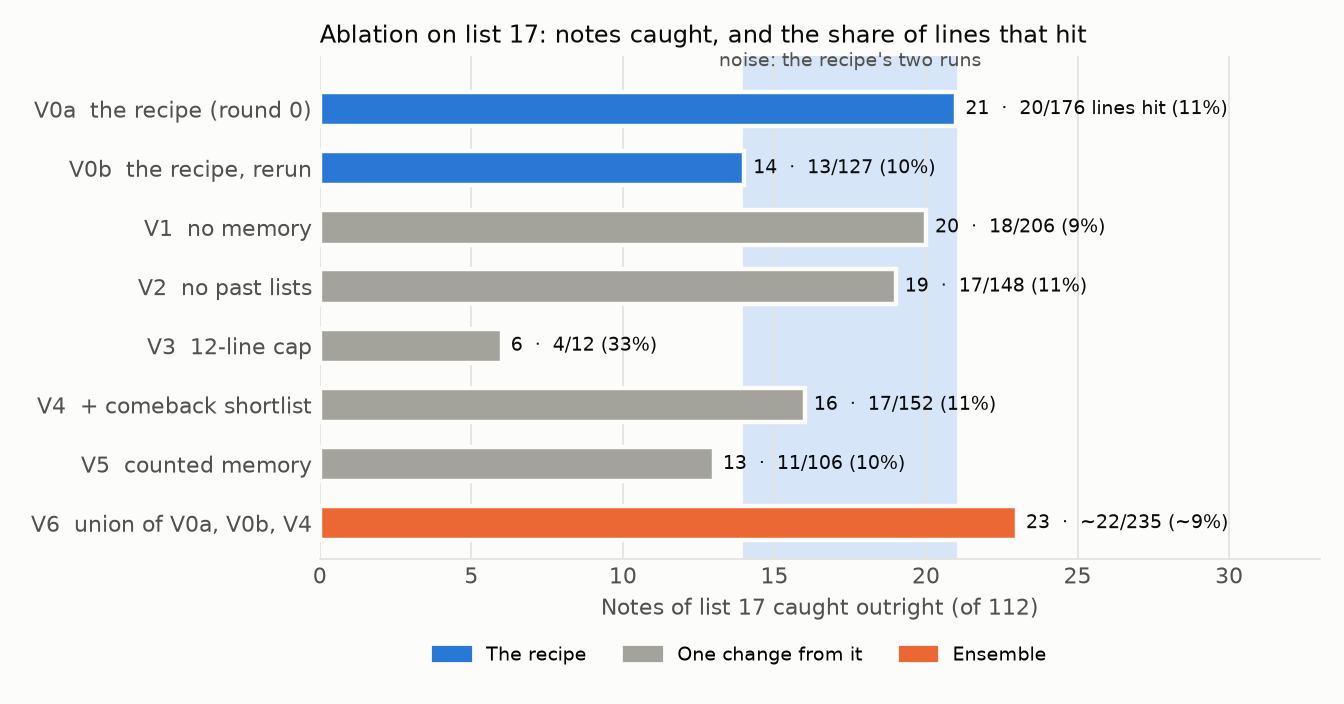
\includegraphics[width=\linewidth]{figures/ablation.png}
  \caption{Ablation on list 17. The shaded band spans the recipe's two runs, 14 to 21 notes: run-to-run noise. Every single change lands inside it except the cap, which trades notes for precision. Pooling three runs (orange) is the only variant above the band.}
  \label{fig:ablation}
\end{figure}

What it showed:
\begin{itemize}[leftmargin=*]
  \item \textbf{Noise is as big as every effect.} The same recipe scored 21 and then 14. With 112 notes, one standard error at this rate is about four notes. No memory (20), no past lists (19), the shortlist (16) and the counted memory (13) all fall inside the recipe's band, so on one list none can be called better or worse.
  \item \textbf{The todo carries most of what can be forecast.} Removing the memory or the past lists barely moved recall: the todo already says what was built, what was fixed only by a test, and what waits on the developer. This qualifies the held-out result above, where raw lists beat a rules-only memory. That compared two weak setups on other lists.
  \item \textbf{Retrieval-first didn't catch more repeats here.} The shortlist script (FixCache-style recency and repeat counts \citep{kim2007predicting}, with an inverse-frequency weight) fed 89 of V4's 152 lines, but V4 caught 3 of 8 repeats, the same as the recipe. Its extraction was crude: generic words ranked high, and the repeats were mostly already in the todo.
  \item \textbf{The counted memory ranked its rules sensibly but didn't add notes.} After a walk over pairs 02--16 with ExpeL- and ACE-style operations \citep{zhao2024expel, zhang2026ace}, its top rule was ``things fixed but never played come back'' (18 helped, 1 misled). It tied for the most repeats caught, 4 of 8, but caught 13 notes in all.
  \item \textbf{The cap is the one clear effect, and it is a trade.} Twelve lines caught 6 notes at 33\% precision, three times the uncapped runs. In the Second Rite every line becomes work, so precision matters there. A forecast meant to catch oversights wants recall.
  \item \textbf{Pooling runs raises recall.} The union of three runs caught 23, the most of any variant, because each run misses different notes. That is the ensembling effect seen in forecasting \citep{halawi2024approaching}. Notes caught by at least two runs (16) were no better than a single run.
\end{itemize}
One note, the llama's graze, may have leaked to the reruns through a recent commit subject in the agents' start-up context. Every variant caught it, and it also appears in list 16. Dropping it takes one from every row and changes no conclusion. The ablation cost about 1.1M tokens, with no GPU or engine.

\section{Discussion}

\paragraph{Leaks are easy to make and hard to see.} We found five during the work:
\begin{itemize}[leftmargin=*]
  \item a commit subject that named a note before it was written;
  \item early commits that held a list together with its own triage;
  \item an agent counting the lines of label files before forecasting;
  \item a todo that triaged the list being scored;
  \item a memory that stored the labels.
\end{itemize}
Only the last one moved the headline number much, and only a scorer asked to look for recall caught it.

\paragraph{Weights versus context.} In this setting, the context window does more than the weights. A short memory of how the developer reacts helps, but the specifics that score come from reading the history at forecast time. That argues for a memory that says \emph{how} to read the history, not one that summarises it. CIPHER makes the opposite trade for cost, distilling edits into short descriptions because they make a shorter prompt than the edits themselves \citep{gao2024aligning}. With a history this small, the raw lists fit, and the trade isn't needed yet.

\paragraph{Onboarding cost.} A fresh agent per epoch is what keeps an epoch blind, and it's also expensive: each one reads about 200k tokens of todos and lists before it writes a line. We kept agent count low and gave each a whole epoch end to end. The developer's framing: ``Just like real life, onboarding is costly.''

\paragraph{Future work.} The ablation reorders what the survey behind Section~2 suggested:
\begin{itemize}[leftmargin=*]
  \item \textbf{Measure noise before anything else.} Every comparison should run each variant at least twice, on more than one list. On list 17 a single rerun moved the score by seven notes.
  \item \textbf{Ensembles,} combined as in event forecasting \citep{halawi2024approaching}. Pooling three runs was the only change that raised recall. It costs tokens and nothing else.
  \item \textbf{Two lists from one forecast.} A capped ``sure'' list for the Second Rite, where every line becomes work, and an uncapped one for catching oversights.
  \item \textbf{Retrieval first, with better extraction.} The shortlist didn't help on list 17, but its script was crude. The ideas behind it (recency and repeat counts \citep{kim2007predicting, salemi2024lamp}, and retrieval of the most similar past contexts \citep{gao2024aligning, suzgun2026dynamic}) deserve a retest that extracts named things only.
  \item \textbf{A counted memory} \citep{zhang2026ace, zhao2024expel}, retested on list 18. Its counts already rank rules by evidence, which is useful for pruning even where it adds no notes.
  \item \textbf{A judge from another family,} or the hand-checked sample the ablation produced, to calibrate the scorer \citep{panickssery2024llm}.
  \item \textbf{A population of memories} on a Pareto front, as in GEPA \citep{agrawal2026gepa}, only if a single memory plateaus once noise is measured.
\end{itemize}

\paragraph{Limitations.} One developer, one game, seventeen lists. The forecaster and the scorer are the same model family, and the scorer's recall estimate is a judgement call. Much of the training data was seen while the first memory was written, so every in-sample number is optimistic. The held-out set is three lists, plus list 17. The Second Rite's later rounds were never played, so only round~0 has a real-world score. Above all, single runs are noisy: the recipe scored 21 and 14 on the same inputs, so every one-run comparison in this paper carries an error of several notes.

\section{Conclusion}

The First Rite can be run as training, but its curve lies unless recall is measured. Once the labels are kept out of the memory, what remains is a modest, honest prior plus a strong reliance on raw history. The Second Rite turns that prior into work. On the first list no part of the pipeline had seen, the prescribed forecast caught 18.8\% of the developer's notes outright. An ablation then showed how noisy one run is, and that pooling runs is the surest way to catch more. Whether the machine spirit is appeased will be known when a build of the converged todo is played.

\paragraph{Acknowledgements.} The experiments were run by Claude Opus 5.5 agents in Claude Code. The developer supplied every playtest note and every correction to the method.

\bibliographystyle{plainnat}
\bibliography{refs}

\end{document}
